\documentclass[11pt,a4paper]{article}

% ---------- packages ----------
\usepackage[utf8]{inputenc}
\usepackage[T1]{fontenc}
\usepackage[margin=2.2cm]{geometry}
\usepackage{xcolor}
\usepackage{amssymb}
\usepackage{booktabs}
\usepackage{enumitem}
\usepackage{listings}
\usepackage{tikz}
\usetikzlibrary{arrows.meta,positioning,calc,shapes.geometric,backgrounds,fit}
\usepackage[colorlinks=true,linkcolor=blue!50!black,urlcolor=blue!50!black]{hyperref}

% ---------- colours ----------
\definecolor{coldblue}{RGB}{30,120,200}
\definecolor{hotred}{RGB}{200,50,40}
\definecolor{metal}{RGB}{150,150,160}
\definecolor{boxblue}{RGB}{225,238,250}
\definecolor{boxgreen}{RGB}{225,245,228}
\definecolor{boxorange}{RGB}{252,237,213}

% ---------- styles ----------
\tikzset{
  block/.style={draw,rounded corners,minimum width=2.7cm,minimum height=1.1cm,align=center,font=\small,fill=boxblue},
  sens/.style ={draw,rounded corners,minimum width=2.7cm,minimum height=1.1cm,align=center,font=\small,fill=boxgreen},
  st/.style   ={draw,rounded corners,minimum width=1.9cm,minimum height=0.9cm,align=center,font=\scriptsize,fill=boxorange},
  flow/.style ={-{Latex[length=2.5mm]},thick},
  lbl/.style  ={font=\scriptsize,fill=white,inner sep=1pt,align=center}
}

\lstdefinestyle{ino}{
  language=C++,basicstyle=\ttfamily\footnotesize,keywordstyle=\color{blue!70!black}\bfseries,
  commentstyle=\color{green!45!black}\itshape,numbers=left,numberstyle=\tiny\color{gray},
  breaklines=true,frame=single,framesep=4pt,rulecolor=\color{gray!50},showstringspaces=false,tabsize=2
}

\newsavebox{\gbbox}
\newenvironment{checkbox}[1]
  {\par\medskip\noindent\begin{lrbox}{\gbbox}\begin{minipage}{0.95\linewidth}\footnotesize\textbf{#1}\par\smallskip}
  {\end{minipage}\end{lrbox}\setlength{\fboxsep}{8pt}\fcolorbox{red!60!black}{red!5}{\usebox{\gbbox}}\par\medskip}
\newenvironment{tipbox}[1]
  {\par\medskip\noindent\begin{lrbox}{\gbbox}\begin{minipage}{0.95\linewidth}\footnotesize\textbf{#1}\par\smallskip}
  {\end{minipage}\end{lrbox}\setlength{\fboxsep}{8pt}\fcolorbox{green!45!black}{green!5}{\usebox{\gbbox}}\par\medskip}

\newcommand{\warn}{\textcolor{orange!80!black}{$\triangle$}}
\newcommand{\reuse}{\textcolor{green!50!black}{\textbf{[REUSE]}}}
\newcommand{\addp}{\textcolor{orange!85!black}{\textbf{[ADD]}}}
\newcommand{\change}{\textcolor{blue!70!black}{\textbf{[CHANGE]}}}

\title{\vspace{-1.5cm}\textbf{Full Project Build Guide}\\[3pt]
\large The complete two-rail PV-cleaning robot, built step by step ---\\[2pt]
\large reusing the parts you already bought, changing only what must change}
\author{Graduation Project --- prototype phase}
\date{17 June 2026}

\begin{document}
\maketitle
\vspace{-0.5cm}

\noindent\fbox{\parbox{0.98\linewidth}{\small
\textbf{How to read this.} This is the full robot build, written like the bench guide --- small steps,
plain words. Every step is tagged so you know what to do with the parts you already own:
\reuse\ keep the part you bought, \change\ swap or upgrade it, \addp\ buy something new. The aim is to
change \emph{only} what the real robot truly needs.}}

\tableofcontents

% ============================================================
\section{The one table that matters: reuse / change / add}

You already bought most of a working robot. Here is exactly what carries over, what changes, and the few
new things to buy. Everything below in the guide refers back to this.

\begin{center}\footnotesize
\begin{tabular}{@{}p{2.9cm}p{3.5cm}p{2.0cm}p{6.0cm}@{}}
\toprule
\textbf{Subsystem} & \textbf{What you bought} & \textbf{Verdict} & \textbf{What to do} \\
\midrule
Rails & 2$\times$ 2040 V-slot, 1 m & \reuse & Use both as parallel rails. (For a real full panel you'll later want 2.4 m lengths.) \\
Carriage & 1 gantry plate + wheels & \addp & Add a 2nd side for rail 2 --- a bought plate \emph{or} a DIY V-wheel bogie --- plus a cross-beam. \\
Drive motor & 1$\times$ GA25-370 (250 rpm) & \addp & Need \textbf{two} driven rails $\Rightarrow$ add one more GA25-370 (the 1:71 / 60 rpm ratio is ideal). \\
Drive method & GT2 belt + pulleys + idler & \change & Belt is fine on the flat bench. To climb 24$^\circ$ glass, add a \textbf{rack + 2 pinions} (positive drive). \\
Motor driver & L298N (dual H-bridge) & \reuse & Its two channels drive both rail motors. Upgrade to \textbf{Cytron MDD3A} only for the brake-hold on the slope. \\
Brush & 2$\times$ 8/22 bearings & \addp & Add a \textbf{3rd GA25-370} (brush motor) + a 0.96 m roller core + microfibre sleeve. \\
Brush/pump switch & IRF540N $\times$6 + 2N2222 $\times$5 & \reuse & 2N2222 drives the IRF540N gate (or buy IRLZ44N). \\
Water pump & 1$\times$ diaphragm pump & \reuse & + your PVC tube; \addp\ spray bar + flat-fan nozzles + a tank. \\
TEC tiles & 4$\times$ TEC1-12706 & \reuse & Prove water on 4. The full dock scales to 38 (deployment only). \\
TEC cooling & 4$\times$ 40 mm 5 V fans & \change & Use these on the \emph{cold} side. \addp\ hot-side heatsinks + paste + cold plate + a $\geq$24 A 12 V PSU. \\
Sensors & DHT22, DS18B20$\times$2, ACS712, NTC, resistors & \reuse & \addp\ an \textbf{MPU-6050} IMU (tilt / fall detection). \\
Compute & ESP32 & \reuse & \addp\ a \textbf{Raspberry Pi 4} for autonomy; the ESP32 becomes its real-time helper. \\
Logic power & buck 12$\to$5 V & \reuse & Unchanged --- it is your 5 V rail. \\
Carriage power & (bench is tethered) & \addp & For untethered runs add a \textbf{12 V 10 Ah LiFePO\textsubscript{4}} battery. Bench can stay on the wall PSU. \\
Hold on tilt & --- & \addp & MDD3A brake mode + a sprung rack detent (or a self-locking JGY-370 worm motor). \\
Structure & 4 L-brackets, 16 T-nuts & \reuse & + a cross-beam and a chassis plate. \\
\bottomrule
\end{tabular}
\end{center}

\begin{tipbox}{The short version}
Almost everything you bought stays. The real ``new spend'' is: \textbf{2 more GA25-370 motors} (one for
the 2nd rail, one for the brush), the \textbf{rack + pinions}, the \textbf{2nd carriage side + cross-beam},
the \textbf{hot-side cooling + big PSU}, a \textbf{Raspberry Pi 4}, an \textbf{IMU}, and a \textbf{battery}.
Nothing you bought is wasted.
\end{tipbox}

% ============================================================
\section{New words (on top of the bench guide's glossary)}

\begin{description}[leftmargin=2.4cm,style=nextline,itemsep=2pt]
  \item[Rack \& pinion] A fixed toothed strip (rack) and a toothed gear (pinion) on the motor. The teeth
  mesh, so the robot climbs without slipping --- unlike a wheel on glass.
  \item[Gantry / cross-beam] The bar that bridges the two rails; the cart is this beam plus a plate on
  each rail.
  \item[Raspberry Pi 4] A small full computer (the ``big brain'') that plans the job and runs the
  sequence. The ESP32 stays as the fast ``small brain'' for motors and sensors.
  \item[micro-ROS] The link that lets the ESP32 talk to the Raspberry Pi over USB.
  \item[IMU (MPU-6050)] A tilt/motion sensor; tells the robot its angle and trips a stop if it is falling.
  \item[LiFePO\textsubscript{4} battery] A safe rechargeable battery chemistry; powers the carriage so it
  runs without a wall cable.
  \item[Brake mode] A driver setting that shorts the motor windings at rest so the carriage holds on the
  slope instead of creeping down.
\end{description}

% ============================================================
\section{Tools \& the new parts to gather}

\textbf{Reuse all the bench tools} (screwdrivers, Allen keys, jumper wires, multimeter, marker, ruler).
\textbf{New parts to buy} for the full robot (prices in \texttt{MARKET\_PARTS\_BUYLIST.md} /
\texttt{MINIMUM\_PROTOTYPE\_BUYLIST.md}):

\begin{itemize}[leftmargin=*,itemsep=1pt]
  \item 2$\times$ GA25-370 gearmotor (1 for rail 2, 1 for the brush) \addp
  \item Rack (module-1) + 2 pinions (\O30, module-1, 6 mm bore) --- the one \textbf{import} \addp
  \item 2nd carriage side (gantry plate \emph{or} V-wheels + bracket) + a cross-beam \addp
  \item Hot-side heatsinks $\times$4 + thermal paste + Al cold plate + a 12 V $\geq$24 A PSU \addp
  \item 0.96 m brush roller core + microfibre; spray bar + flat-fan nozzles; 5 L tank + fittings \addp
  \item Raspberry Pi 4 (4 GB) + SD card; MPU-6050 IMU; 12 V 10 Ah LiFePO\textsubscript{4} battery \addp
  \item (Optional, better hold/brake) Cytron MDD3A driver \addp
\end{itemize}

% ============================================================
\section{Step A --- the two rails (twin-rail base)}

Same idea as the bench's twin-rail step, now the backbone of the real robot: two parallel rails, a gantry
plate on each, a cross-beam joining them, only \textbf{rail 1 driven}.

\begin{figure}[h]
\centering
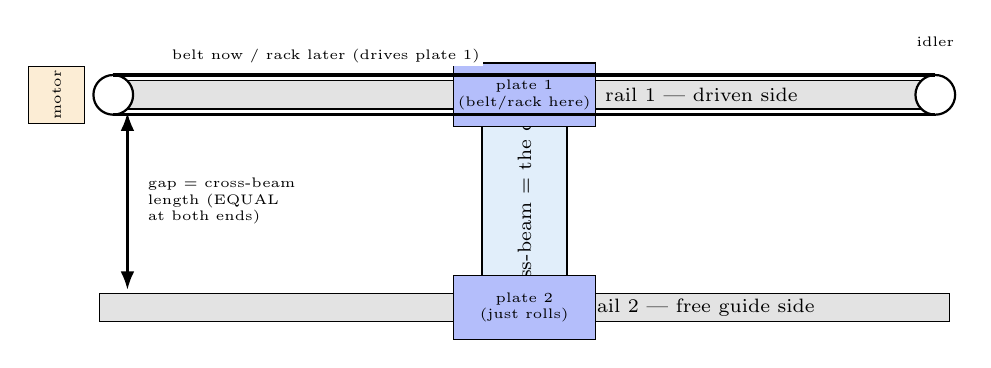
\begin{tikzpicture}[scale=0.9]
\fill[gray!22] (0,2.8) rectangle (12,3.2); \draw (0,2.8) rectangle (12,3.2);
\node[font=\scriptsize] at (8.5,3.0){rail 1 --- driven side};
\fill[gray!22] (0,-0.2) rectangle (12,0.2); \draw (0,-0.2) rectangle (12,0.2);
\node[font=\scriptsize] at (8.5,0.0){rail 2 --- free guide side};
\fill[boxblue] (5.4,0) rectangle (6.6,3.0); \draw[thick] (5.4,0) rectangle (6.6,3.0);
\node[font=\scriptsize,align=center,rotate=90] at (6.0,1.5){cross-beam = the cart};
\fill[boxblue!80!blue] (5.0,2.55) rectangle (7.0,3.45); \draw (5.0,2.55) rectangle (7.0,3.45);
\node[font=\tiny,align=center] at (6.0,3.0){plate 1\\(belt/rack here)};
\fill[boxblue!80!blue] (5.0,-0.45) rectangle (7.0,0.45); \draw (5.0,-0.45) rectangle (7.0,0.45);
\node[font=\tiny,align=center] at (6.0,0.0){plate 2\\(just rolls)};
\fill[boxorange] (-1.0,2.6) rectangle (-0.2,3.4); \draw (-1.0,2.6) rectangle (-0.2,3.4);
\node[font=\tiny,align=center,rotate=90] at (-0.6,3.0){motor};
\draw[thick,fill=white] (0.2,3) circle (0.28); \draw[thick,fill=white] (11.8,3) circle (0.28);
\node[font=\tiny] at (11.8,3.75){idler};
\draw[very thick] (0.2,3.28)--(11.8,3.28); \draw[very thick] (0.2,2.72)--(11.8,2.72);
\node[font=\tiny,fill=white,inner sep=1pt] at (3.2,3.55){belt now / rack later (drives plate 1)};
\draw[{Latex}-{Latex},thick] (0.4,0.25)--(0.4,2.75);
\node[font=\tiny,align=left,right] at (0.55,1.5){gap = cross-beam\\length (EQUAL\\at both ends)};
\end{tikzpicture}
\caption{The twin-rail base (reused from the bench). Build and test this flat first with the belt; the
rack-and-pinion replaces the belt for climbing (Step C).}
\end{figure}

\reuse\ both rails, the gantry plate, T-nuts, L-brackets, belt+pulleys+idler. \addp\ the 2nd carriage
side + cross-beam. Follow Steps~1--11 of the bench guide (\texttt{guide.pdf}, Step group A) --- they are
identical here.

% ============================================================
\section{Step B --- the climbing drive: add rack-and-pinion}

\change\ The belt drives the cart fine on a flat table, but \textbf{cannot climb 24$^\circ$ glass}. For
the real panel you add a rack-and-pinion: teeth that mesh, so the drive cannot slip.

\begin{figure}[h]
\centering
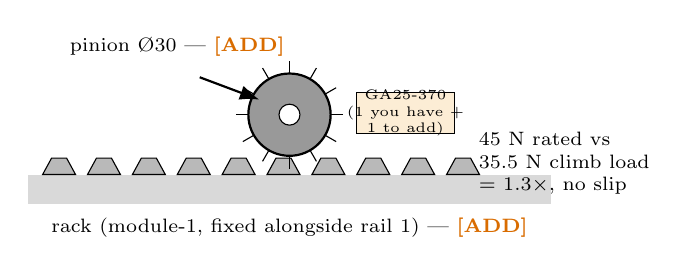
\begin{tikzpicture}[scale=0.95]
\fill[gray!30] (0,0) rectangle (7,0.4);
\foreach \x in {0.2,0.8,...,6.2}{\draw[fill=gray!55] (\x,0.4)--(\x+0.12,0.62)--(\x+0.32,0.62)--(\x+0.44,0.4)--cycle;}
\node[font=\scriptsize,below] at (3.5,-0.05){rack (module-1, fixed alongside rail 1) --- \addp};
\draw[thick,fill=gray!80] (3.5,1.2) circle (0.55);
\foreach \a in {0,30,...,330}{\draw[fill=gray!60] (3.5,1.2)++(\a:0.55)--++(\a:0.17);}
\draw[fill=white] (3.5,1.2) circle (0.14);
\node[font=\scriptsize,above] at (2.0,1.85){pinion \O30 --- \addp};
\draw[flow] (2.3,1.7)--(3.1,1.4);
\fill[boxorange] (4.4,0.95) rectangle (5.7,1.5); \draw (4.4,0.95) rectangle (5.7,1.5);
\node[font=\tiny,align=center] at (5.05,1.22){GA25-370\\(1 you have +\\1 to add)};
\node[font=\scriptsize,align=left,right] at (5.9,0.55){45 N rated vs\\35.5 N climb load\\$=$ 1.3$\times$, no slip};
\end{tikzpicture}
\caption{Add a module-1 rack alongside rail 1 and a \O30 pinion on each drive motor. Two driven rails
$\Rightarrow$ two GA25-370 motors (you have one, add one). Drive both from the L298N's two channels.}
\end{figure}

\begin{checkbox}{\warn\ Hold the carriage on the slope}
A GA25-370 is not self-locking, so it would creep down when stopped. Use the \textbf{MDD3A brake mode}
(\addp, the upgrade from the L298N) plus a sprung detent in the rack, or swap to a self-locking
\textbf{JGY-370} worm motor. On the flat bench you can ignore this.
\end{checkbox}

\reuse\ your GA25-370, the L298N (drives both rail motors), the ESP32. \addp\ a 2nd GA25-370, the rack,
two pinions, and (for the brake-hold) the MDD3A.

% ============================================================
\section{Step C --- the full-width brush + spray}

\addp\ a \textbf{3rd GA25-370} to spin a $\approx$0.96 m microfibre roller (your 8/22 bearings carry its
ends). \reuse\ your pump and PVC tube; \addp\ a spray bar + nozzles + tank. Switch the brush motor and
pump with your IRF540N + 2N2222 driver (or IRLZ44N).

\begin{figure}[h]
\centering
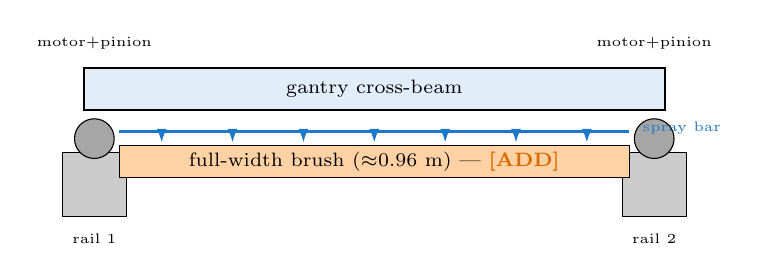
\begin{tikzpicture}[scale=0.9]
\fill[gray!40] (-0.4,0) rectangle (0.5,0.9); \draw(-0.4,0) rectangle (0.5,0.9); \node[font=\tiny,below] at (0.05,-0.1){rail 1};
\fill[gray!40] (7.5,0) rectangle (8.4,0.9); \draw(7.5,0) rectangle (8.4,0.9); \node[font=\tiny,below] at (7.95,-0.1){rail 2};
\fill[boxblue] (-0.1,1.5) rectangle (8.1,2.1); \draw[thick] (-0.1,1.5) rectangle (8.1,2.1);
\node[font=\scriptsize] at (4.0,1.8){gantry cross-beam};
\draw[fill=gray!70] (0.05,1.1) circle (0.28); \draw[fill=gray!70] (7.95,1.1) circle (0.28);
\node[font=\tiny,align=center] at (0.05,2.45){motor+pinion}; \node[font=\tiny,align=center] at (7.95,2.45){motor+pinion};
\fill[orange!35] (0.4,0.55) rectangle (7.6,1.0); \draw (0.4,0.55) rectangle (7.6,1.0);
\node[font=\scriptsize] at (4.0,0.78){full-width brush ($\approx$0.96 m) --- \addp};
\draw[very thick,coldblue] (0.4,1.2)--(7.6,1.2);
\foreach \x in {1,2,...,7}{\draw[-{Latex},coldblue] (\x,1.2)--(\x,1.05);}
\node[font=\tiny,coldblue,right] at (7.65,1.25){spray bar};
\end{tikzpicture}
\caption{Front view. Brush, spray bar, tank and battery hang on the cross-beam; each rail end is driven.}
\end{figure}

% ============================================================
\section{Step D --- water from the air (your 4 tiles)}

\reuse\ the 4 TEC tiles and the 40 mm fans (now on the cold side). \change\ the cooling: \addp\ hot-side
heatsinks + paste + a cold plate + a $\geq$24 A 12 V PSU --- exactly the bench harvest step. Prove water
on 4 tiles; the 38-tile, 48 V dock is deployment-only.

\begin{figure}[h]
\centering
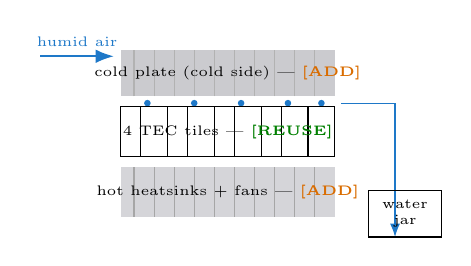
\begin{tikzpicture}[scale=0.85]
\draw[-{Latex},coldblue,thick] (-1.0,3.0)--(0.1,3.0); \node[font=\tiny,coldblue,above] at (-0.45,3.0){humid air};
\fill[metal!50] (0.2,2.4) rectangle (3.4,3.1); \foreach \x in {0.4,0.7,...,3.2}{\draw[gray!60](\x,2.4)--(\x,3.1);}
\node[font=\tiny] at (1.8,2.75){cold plate (cold side) --- \addp};
\foreach \x in {0.6,1.3,2.0,2.7,3.2}{\fill[coldblue] (\x,2.3) circle (1.4pt);}
\fill[white] (0.2,1.5) rectangle (3.4,2.25); \draw (0.2,1.5) rectangle (3.4,2.25);
\foreach \x in {0.7,1.4,2.1,2.8}{\draw (\x-0.2,1.5) rectangle (\x+0.2,2.25);}
\node[font=\tiny] at (1.8,1.87){4 TEC tiles --- \reuse};
\fill[metal!40] (0.2,0.6) rectangle (3.4,1.35); \foreach \x in {0.4,0.7,...,3.2}{\draw[gray!70](\x,0.6)--(\x,1.35);}
\node[font=\tiny] at (1.8,0.97){hot heatsinks + fans --- \addp};
\draw[-{Latex},coldblue] (3.5,2.3)--(4.3,2.3)--(4.3,0.3);
\draw (3.9,0.3) rectangle (5.0,1.0); \node[font=\tiny,align=center] at (4.45,0.65){water\\jar};
\end{tikzpicture}
\caption{The harvest stack. Identical physics to the bench: cold plate up (water forms), hot heatsink +
fans down. Your 40 mm fans move humid air across the cold side.}
\end{figure}

% ============================================================
\section{Step E --- sensors, brains, power, autonomy}

\reuse\ DHT22, DS18B20, ACS712, and the encoders in the motors. \addp\ an \textbf{MPU-6050} (tilt/fall),
a \textbf{Raspberry Pi 4} (the planner), and a \textbf{12 V 10 Ah battery} so the cart runs untethered.
The ESP32 stays as the real-time helper.

\begin{figure}[h]
\centering
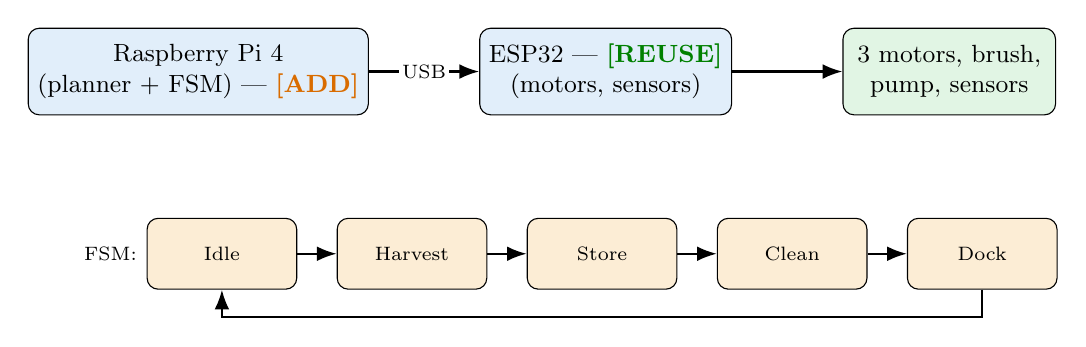
\begin{tikzpicture}[node distance=0.8cm and 1.4cm]
\node[block](pi){Raspberry Pi 4\\(planner + FSM) --- \addp};
\node[block,right=of pi](esp){ESP32 --- \reuse\\(motors, sensors)};
\node[sens,right=of esp](io){3 motors, brush,\\pump, sensors};
\draw[flow] (pi)--node[lbl]{USB}(esp); \draw[flow] (esp)--(io);
\node[st,below=1.3cm of pi.south,xshift=0.3cm](idle){Idle};
\node[st,right=0.5cm of idle](harv){Harvest};
\node[st,right=0.5cm of harv](store){Store};
\node[st,right=0.5cm of store](clean){Clean};
\node[st,right=0.5cm of clean](dock){Dock};
\draw[flow](idle)--(harv);\draw[flow](harv)--(store);\draw[flow](store)--(clean);\draw[flow](clean)--(dock);
\draw[flow](dock.south)--++(0,-0.35)-|(idle.south);
\node[font=\scriptsize,left] at (idle.west){FSM:};
\end{tikzpicture}
\caption{Two-brain control. The Pi runs the Idle$\to$Harvest$\to$Store$\to$Clean$\to$Dock cycle; the
ESP32 (yours) does the fast motor/sensor work.}
\end{figure}

\paragraph{Code changes from the bench sketch.} The bench sketch drove one motor. Now drive \textbf{two}
rail motors on the L298N's two channels (ENA/IN1/IN2 \emph{and} ENB/IN3/IN4), add the brush motor + pump
on switched pins, read the IMU, and let the Pi command the sweep over serial. Pin map to add:

\begin{center}\small
\begin{tabular}{@{}lll@{}}
\toprule
Function & ESP32 pin(s) & Note \\
\midrule
Drive motor 1 & ENA 25 / IN1 26 / IN2 27 & \reuse\ from bench \\
Drive motor 2 & ENB 14 / IN3 12 / IN4 13 & \addp\ 2nd channel of L298N \\
Brush motor on/off & GPIO 4 $\to$ 2N2222 $\to$ IRF540N & \reuse\ your MOSFET driver \\
Pump on/off & GPIO 16 $\to$ 2N2222 $\to$ IRF540N & \reuse \\
IMU (MPU-6050) & SDA 21 / SCL 22 (I\textsuperscript{2}C) & \addp \\
Pi link & USB serial & \addp\ micro-ROS \\
\bottomrule
\end{tabular}
\end{center}

% ============================================================
\section{Build order \& test plan}

\begin{enumerate}[leftmargin=*,itemsep=2pt]
  \item Build the twin-rail base flat and run the bench motion test \textbf{with the belt} (proves the
  cart + code + encoders). \reuse\ everything.
  \item Add the 2nd drive motor; drive both from the L298N; re-test on the flat.
  \item Add the rack + pinions; tilt the rails and prove the \textbf{climb} up and down with brake-hold.
  \item Add the brush motor + roller, then the spray bar + pump + tank.
  \item Build the TEC harvest stack on 4 tiles; weigh the water.
  \item Add the IMU and the battery; cut the wall tether.
  \item Add the Raspberry Pi; bring up odometry (encoder + IMU) and the limit-switch re-zero.
  \item Run the full Idle$\to$Dock state machine.
\end{enumerate}

\begin{tipbox}{Why this order is safe}
Each step adds one block to a thing that already works. You never debug two new things at once. Steps 1--2
are your current bench; everything after is one \addp\ at a time.
\end{tipbox}

% ============================================================
\section{What to buy}

The priced lists are already done: \texttt{MINIMUM\_PROTOTYPE\_BUYLIST.md} (bench, with your purchases
marked) and \texttt{MARKET\_PARTS\_BUYLIST.md} (full robot + residential dock). This guide's
\addp\ items map directly onto the ``Still needed'' sections there.

\vspace{0.3cm}
\noindent\fbox{\parbox{0.98\linewidth}{\small\textbf{In one line:} keep everything you bought, add two
motors + a rack-and-pinion + a second brain + a battery + hot-side cooling, and build it one tested block
at a time. The bench you have is the first two blocks of the real robot.}}

\end{document}
